\documentclass{article}
\usepackage{graphicx} 
\usepackage{caption}
\usepackage{multicol}
\usepackage{algorithmic}
\usepackage[letter]{geometry}
\usepackage{float}
\setlength{\columnsep}{1cm}
\usepackage[
backend=biber, 
style=apa
]{biblatex}
\addbibresource{references.bib}

\title{Flare Finder}
\author{Sophia Wang}
\date{July 2024}

\begin{document}
\begin{center}
    \Large
    \textbf{Flare Finder: Detecting Near-Ultraviolet Flares in M-dwarfs in Swift UVOT Event Data} \\
    \vspace{1cm}
    \large
    Sophia Wang \\
    Institute for Computing in Research \\
    July 2024 \\
    \vspace{1cm}
    
    \Large
    \textbf{Abstract}
    
\end{center}
This paper discusses the algorithms and usage of Flare Finder, a program developed to detect near-ultraviolet (NUV) flares on M dwarfs from data from the Neil Gehrels Swift Observatory (\textit{Swift}). In previous studies, flares on M-dwarfs are first imaged optically, and telescopes encompassing other wavelengths with narrower ranges are turned to record data accordingly; however, NUV flares on M dwarfs do not always produce an optical flare distinguishable from noise, biasing the set of observed flares. Given event data from the \textit{Swift} ultraviolet and optical telescope (UVOT), Flare Finder isolates distinct stars using aperture photometry and, without optical input, identifies candidates for flare stars and timestamps of the flare(s). The program bins data into light curves, and signal-to-noise ratios (SNRs) are calculated for each flare duration window of time for each star. The process is tested using \textit{Swift} UVOT event data of a recent flare on flare star YZ Canis Minoris (YZ CMi) and its results, implications, shortcomings, and possible improvements are discussed.

\vspace{1cm}

\begin{multicols}{2}

\section{Introduction}

Representing about 70\% of all stellar objects, M-dwarfs are characterized by their low mass and long lifespans (\cite{bochanski}). Observations of M-dwarfs have revealed that most are favorable hosts for large systems of exoplanets, including rocky- and Jupiter-sized planets; roughly one-third of rocky planets orbit in the circumstellar habitable zones of M-dwarfs (\cite{aomawa}). M-dwarfs also flare more frequently compared to other stars, as they generate stronger magnetic fields (\cite{shulyak}). Flares occur when stored magnetic energy is converted into kinetic energy and released, heating up the star and causing it to emit radiation observable across the electromagnetic spectrum (\cite{kowalski}). 

Understanding and characterizing stellar flares on M-dwarfs is critical for determining the habitability of orbiting exoplanets, especially near-ultraviolet (NUV) radiation. Giant stellar flares create high levels of UV radiation that alter planetary atmospheres, decreasing habitability (\cite{howard}). On the other hand, certain levels of ultraviolet radiation are essential for prebiotic chemistry, such as ribonucleotides (\cite{ranjan}). 

Typically, NUV wavelength data of M dwarf flares is collected through targeted investigation. Flares are first observed through the optical wavelength using wide-field cameras, for example the Transiting Exoplanet Survey Satellite (TESS); telescopes with smaller fields measuring in different wavelengths are then pointed directly at the identified target, for example the Neil Gehrels Swift Observatory (\textit{Swift}) ultraviolet and optical telescope (UVOT). However, this method of flare detection biases observations against detecting high-energy NUV flares, and only 28\% of NUV flares have an accompanying optical flare, as the flare is diluted in noise in the light curve (\cite{paudel}). Thus, relying on optical data to discover flare stars is insufficient to answer the question of habitability with regard to ultraviolet light. 

This paper introduces a method to programmatically detect flares in \textit{Swift} UVOT event data to fill the gap in detected flares without optical input, and is organized as follows. Section 2 outlines details of the \textit{Swift} UVOT, event data, and flare detection algorithm. The algorithm is run on example data with a known flare occurrence, and the results are discussed in Section 3. Section 4 gives a summary of the main results from this project and future improvements. 

\section{Data and Algorithm}

\subsection{The \textit{Swift} UVOT and Event Data}

The three-telescope \textit{Swift} observatory was launched in 2004 and remains in service today. One of these telescopes is the UVOT, which counts photons in the optical and ultraviolet wavelengths (1600 to 6000 {\AA}) with a timing resolution of approximately 11 ms (\cite{nasaSwiftUVOT}). Due to its limited field of view (17 by 17 arcminutes), to this point, it is intentionally pointed at a known flare star to detect NUV flare data. 

The UVOT saves data in three modes, one of which is Event mode. Event mode saves a list of observed photons, or events, and their timestamps, respective coordinates in three different formats, exposure references, and quality flags (\cite{swiftGuide}). For the Flare Finder algorithm, the data of interest is the timestamp, X and Y position, and quality flag of each event. 

\subsection{Flare Finder Algorithm}

The Flare Finder algorithm first cleans data for quality and contiguity. Events with a nonzero quality flag are removed, as well as events at timestamps with few other observations. The remaining data is processed for star detection, then flare detection. The program was first written using Jupyter notebook software and later converted to a single Python file (\cite{jupyter}).

\subsubsection{Star Detection} \label{sss:starDetect}

During star detection, data is first binned along the X and Y into a 1000 by 1000 2D histogram. Then, synthetic aperture photometry is used to identify individual stars, using a similar but simplified application of the DAOPHOT algorithm (\cite{stetson}). A circular aperture spanning 2 by 2 pixels is used as the window for photon counts of a star, and an annulus aperture with an outer radius of 11 pixels and an inner radius of roughly 9 pixels is used to calculate the local background for that star. 

For every 2 by 2 pixel area on the 2D histogram, the total star counts (\(C_t\)) in the circular aperture are added together, and the background counts (\(C_s\)) are similarly summed. Moreover, the area of the signal and sky apertures are calculated (\(A_t = 4\) and \(A_s = 184\), respectively). The signal in the aperture \(N_t\) is calculated with equation \ref{eq:imgSigAp}.
    
\begin{equation} \label{eq:imgSigAp}
    N_t = C_t - A_t \times \frac{C_s}{A_s}
\end{equation}

The sky background per pixel \(N_s\) is also calculated as:

\begin{equation} \label{eq:skyBgPix}
    N_s = \frac{A_t \times C_s}{A_s}
\end{equation}

Using output from equations \ref{eq:imgSigAp} and \ref{eq:skyBgPix}, the total noise \(\sigma\) is thus calculated as:

\begin{equation} \label{eq:imgTotNoise}
    N = \sqrt{N_t + N_s}
\end{equation}

The final signal-to-noise ratio (SNR) is, naturally, calculated with equation \ref{eq:snr}.

\begin{equation} \label{eq:snr}
    SNR = \frac{N_t}{N}
\end{equation}

After calculation of all SNRs in the image, Flare Finder identifies the mean \(\bar{x}\) and standard deviation \(\sigma\) of the ratios, which by definition are approximately 0 and 1, respectively. Stars, which are bright relative to their local background, by definition have a larger SNR compared to the mean; the algorithm applies a simple threshold of five standard deviations from the mean to isolate stars from the background. That is, for any point $i, j$, if \(SNR_{i, j} > \bar{x} + 5 \times \sigma\), then that point belongs to a star in the original data. 

Following this threshold application, a basic floodfill algorithm is used to determine all points of individual stars. The coordinates and average SNR belonging to each star are saved, and the program continues on to flare detection.

\subsubsection{Flare Detection} \label{sss:flareDetect}

The algorithm for flare detection uses a nested iterative process to search for flares in every star. 

\noindent\makebox[\linewidth]{\rule{\columnwidth}{0.4pt}} 
\textbf{Flare Finding Algorithm}

\begin{algorithmic}
\FOR {\texttt{$star$} in \texttt{$star data$}}
    \STATE {Get star data}
    \FOR {\texttt{$time$ $window$ $length$}}
        \FOR {\texttt{$timestamp$} in \texttt{$star$ $data$}}
            \STATE {$SNR$ $\gets$ {calculated SNR ratio}}
            \RETURN {$SNR$}
        \ENDFOR
        \STATE {$Outliers$ $\gets$ {list of outlier SNRs}}
        \RETURN {$Outliers$}
    \ENDFOR
\ENDFOR
\end{algorithmic}

\noindent\makebox[\linewidth]{\rule{\columnwidth}{0.4pt}}

All in all, there are three for loops to iterate over the star, the length of the time window, and the timestamp in the star data. For each star, the raw data from the UVOT event list is gathered, sorted, and binned into an Astropy TimeSeries with a bin size of one second. That is, all timestamps within the same second will be summed into one bin containing the total number of photon events for that second. The program then iterates over different signal window sizes to accommodate for flares of different lengths, and calculates the SNR for each window of time in the TimeSeries. 

The SNR calculation over the time domain is relatively similar to the calculation for images, but with some noticeable changes. Rather than an annulus and circle, there is a signal window of length \(L_s\), and two background windows to the left and right of that window, with lengths \(L_{bg} = 1.5 \times L_s\). 

\begin{equation} \label{eq:tdBgMeanRate}
    N_bg = \frac{C_{bg}}{L_{bg}}
\end{equation}

Equation \ref{eq:tdBgMeanRate} describes the mean counts per unit time \(N_{bg}\) in the background, where \(C_{bg}\) is the total photon counts in the background. 

\begin{equation} \label{eq:tdSigMeanRate}
    N_s = \frac{C_s}{L_s} - N_{bg}
\end{equation}

Meanwhile, equation \ref{eq:tdSigMeanRate} is the calculation for the mean photon counts in the signal window, subtracting background noise, where \(C_s\) is the total photon counts in the signal window. 

The total noise rate is also calculated using the standard deviation of the events in the background. For each bin $i$ in the background, letting the number of photon events per second in that bin be $x_i$, then the total noise was calculated with equation \ref{eq:tdNoise}.

\begin{equation} \label{eq:tdNoise}
    N = \sqrt{\frac{\sum{(x_i - N_{bg})^2}}{L_{bg}}}
\end{equation}

The SNR is still calculated using the same equation as \ref{eq:snr}. With \(N_s\) still as the mean signal rate, the SNR for a particular time window in a particular star is:

\begin{equation}
    SNR = \frac{N_s}{N}
\end{equation}

Like when detecting stars, the algorithm returns all the timestamps with an extremely high SNR (i.e. \(SNR \geq \bar{x} + 5 \times \sigma\)). The returned timestamps are all candidates of when a flare may have occurred. 

\section{Results}

The Flare Finder algorithm was tested on recently procured \textit{Swift} UVOT event data, including a flare from star YZ Canis Minoris (YZ CMi). The 2D histogram of the event data is shown below (Figure \ref{img:2DHist}). 

\end{multicols}

\begin{figure}[h]
    \centering
    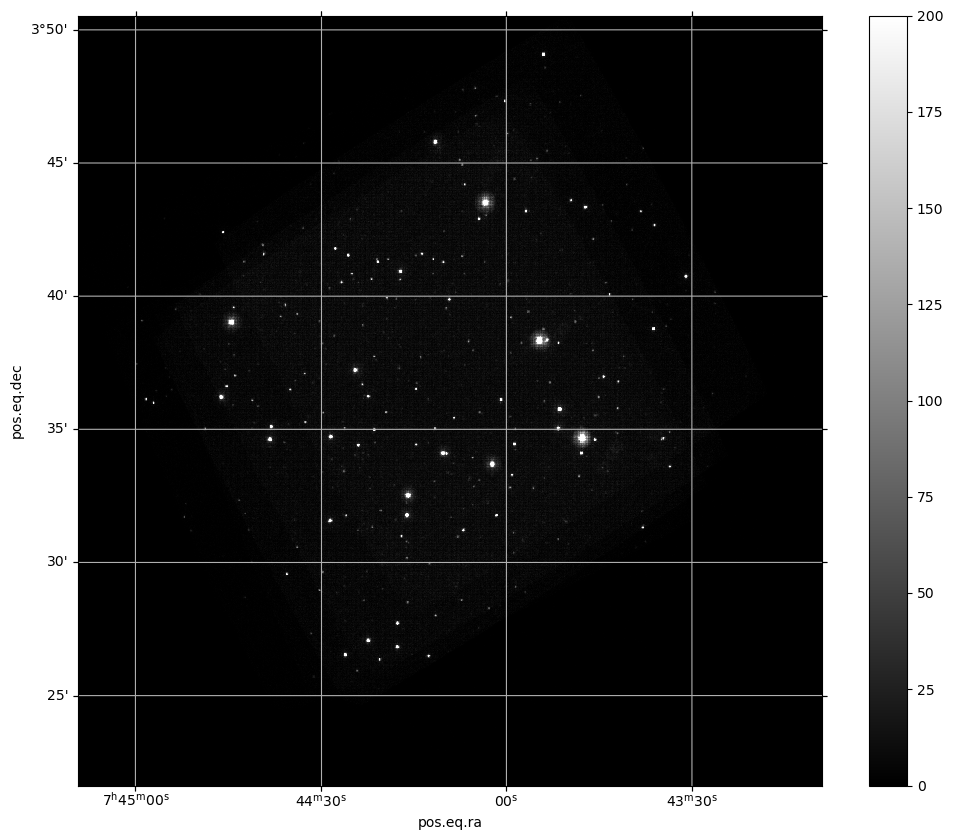
\includegraphics[width=\textwidth]{example2DHist.png}
    \caption{Grayscale 2D histogram of \textit{Swift} UVOT event data.}
    \label{img:2DHist}
\end{figure}

\begin{multicols}{2}

Using the star detection algorithm detailed in Section \ref{sss:starDetect}, the SNRs of each pixel in Figure \ref{img:2DHist} was calculated with the annulus in Figure \ref{img:annulus}. The detected stars were plotted in Figure \ref{img:imgSNR} on the left, while all points above the 5-standard-deviation threshold were plotted on the right.

\end{multicols}

\begin{figure}[h]
    \centering
    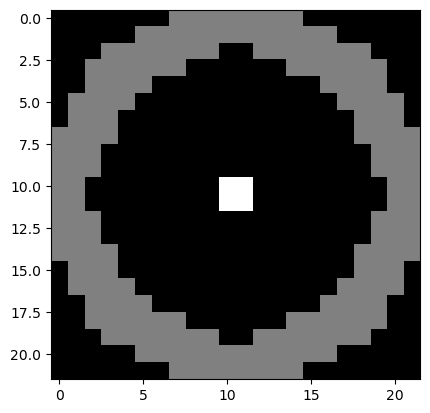
\includegraphics[width=2in]{annulus_png.png}
    \caption{Annulus/circle aperture used for star detection, where the white section is the circle aperture and the gray annulus is the background aperture.}
    \label{img:annulus}
\end{figure}

\begin{figure}[h]
    \centering
    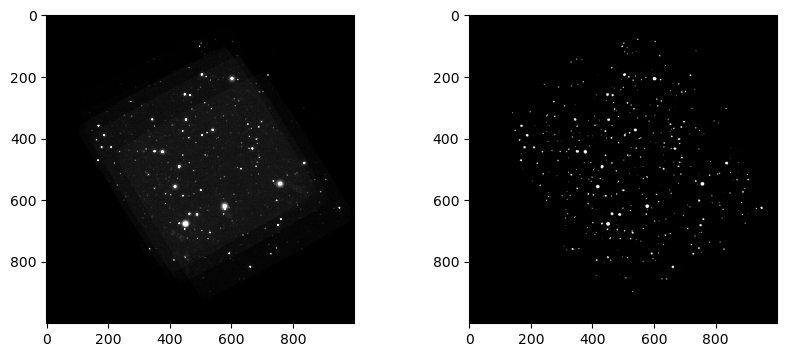
\includegraphics[width=\textwidth]{imgSNR.png}
    \caption{Star data after SNR ratios are calculated. Left: Visualization of SNR ratios of each point on the image. Right: Visualization of all points with SNRs above 5-standard-deviation threshold.}
    \label{img:imgSNR}
\end{figure}

\begin{multicols}{2}

Noticeably, as seen in Figure \ref{img:imgSNR}, on the left, the calculated SNRs of the background are nonzero. Due to limb darkening, the brighter region of each star on the left  is larger than the threshold-cut points on the right. 

To test the Flare Finding algorithm on individual stars, two relatively large and bright stars were selected and analyzed for flares. From this point, the star in Figure 4 will be referred to as star A, and the star in Figure 5 will be referred to as star B.

For both stars, histograms of calculated SNR ratios for time windows of 10 seconds were also generated.

\end{multicols}

\begin{figure}[h]
  \begin{minipage}[b]{.45\linewidth} 
    \centering
    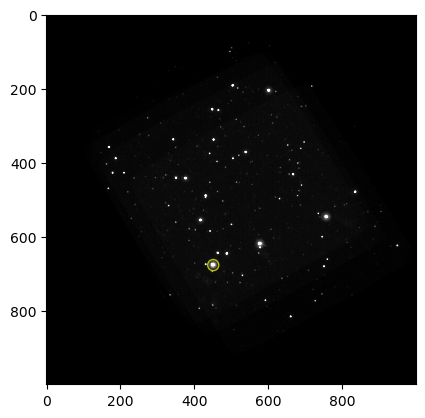
\includegraphics[scale=0.5]{star_333.png}
    \captionof{figure}{Star A.}
  \end{minipage}\hfill
  \begin{minipage}[b]{.45\linewidth}
    \centering
    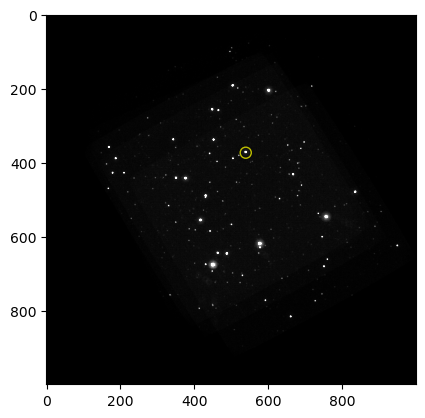
\includegraphics[scale=0.5]{star_109.png}
    \captionof{figure}{Star B.}
  \end{minipage}
\end{figure}

\begin{figure}[h]
    \centering
    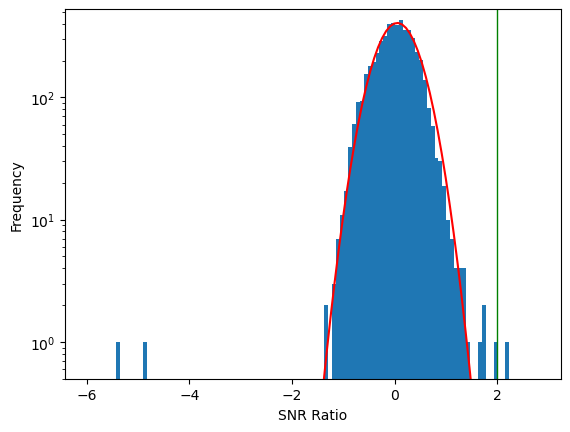
\includegraphics[scale=0.6]{333_hist.png}
    \caption{Histogram of SNR ratios for Star A, with fitted Gaussian curve in red, and vertical bar five standard deviations from the mean in green.}
    \label{img:histA}
\end{figure}

\begin{figure}[t]
    \centering
    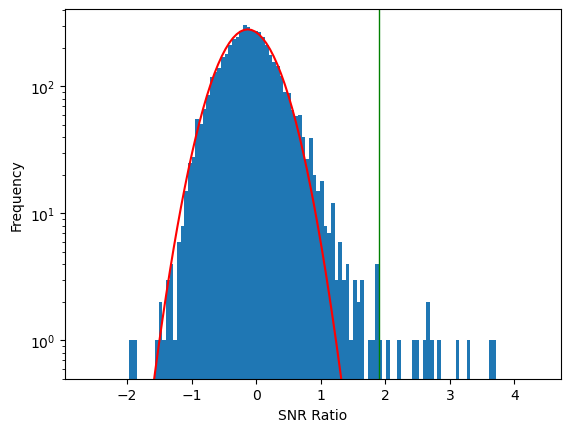
\includegraphics[scale=0.6]{109_hist.png}
    \caption{Histogram of SNR ratios for Star B, with red Gaussian curve and green vertical bar for 5-standard-deviation threshold.}
    \label{img:histB}
\end{figure}

\begin{multicols}{2}

Noticeably in Figure \ref{img:histA}, there are few candidates for flares in a window of 10 seconds for star B. There are also two low outliers with SNRs between -4 and -6 that indicate a large dip in the signal window compared to peaks in the background; i.e. there are more photons detected in the background than in the signal window. Meanwhile in Figure \ref{img:histB}, there are numerous timestamp candidates for flares and no low outliers. 

It is important to note that number of outlier ratios in the histogram does not equal the number of probable flares in the data. Because the actual flare duration may be slightly shorter or longer than the signal window, in this case 10 seconds, multiple consecutive timestamps may be marked as having a flare. 

Figure \ref{img:peakA} shows the timestamp with the largest calculated SNR of about 2.2310. Zooming out in Figure \ref{img:zoomA}, it is clear that while this is a local peak, its height is still relatively similar to the extended background. Moreover, there are two spikes in the TimeSeries where the photon count approaches 60 counts/second, but because the duration of the peak is so short, for a window of 10 seconds, it becomes averaged into the background. Hence, if the signal window length is a poor estimate of the true flare duration, much shorter or longer flares may not be detected at all. 

\end{multicols}

\newpage

\begin{figure}[t]
    \centering
    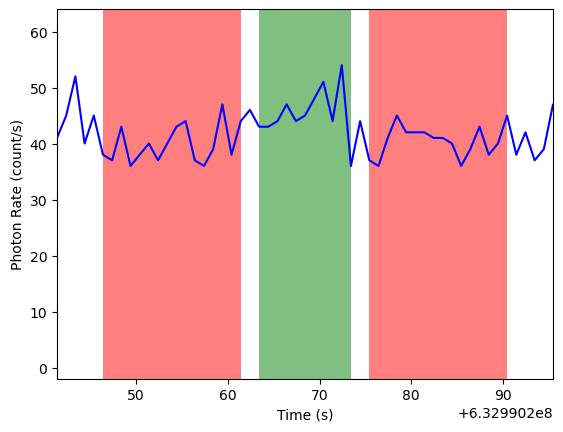
\includegraphics[scale=0.5]{333_ts_peak.png}
    \caption{Relevant TimeSeries visualization for the timestamp with the largest calculated SNR for Star A, where the shaded green region represents the signal window, the two shaded red regions represent the background windows, and the blue line indicates the photon count per second.}
    \label{img:peakA}
\end{figure}

\begin{figure}[h]
    \centering
    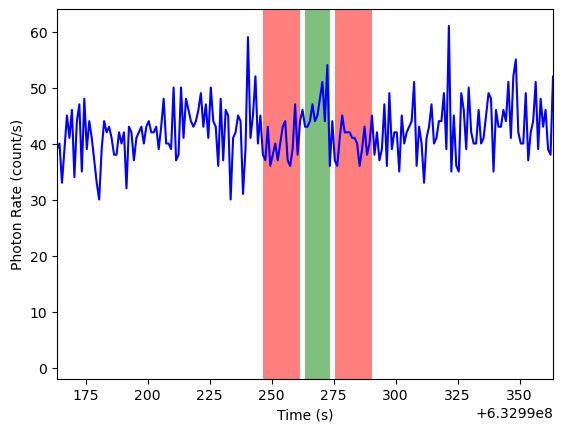
\includegraphics[scale=0.5]{333_ts_zoomout.png}
    \caption{TimeSeries visualization of the peak in Figure \ref{img:peakA}, zoomed out so that there are about 80 seconds before and after the background windows.}
    \label{img:zoomA}
\end{figure}

\begin{multicols}{2}

The largest calculated SNR value for Star B was approximately 3.7143, indicating a very strong signal from the signal window. As seen in Figure 10, there is a dramatic increase at time 633000886, and the maximum photon rate of over 50 photons/second is much larger than the average in the local background mean rate of roughly 15.6333, indicative of a flare. Zooming out in Figure 11 reveals the entirety of the flare, which was largely undetected as the time window of 10 seconds was to short to detect the whole flare. As expected, this is a flare on M-dwarf flare star YZ CMi detected by \citeauthor{paudel} using TESS (\citeyear{paudel}). 

\end{multicols}
\newpage
\begin{figure}[hp]
  \begin{minipage}[b]{.45\linewidth} 
    \centering
    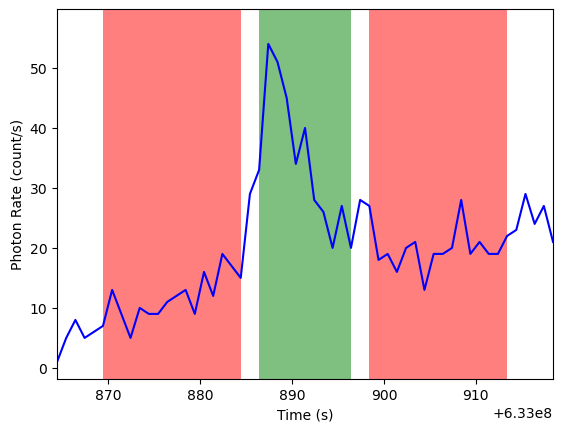
\includegraphics[scale=0.5]{109_ts_peak.png}
    \captionof{figure}{Relevant TimeSeries visualization for the timestamp with the largest calculated SNR for Star B, with a very large spike in the central green signal window.}
  \end{minipage}\hfill
  \begin{minipage}[b]{.45\linewidth}
    \centering
    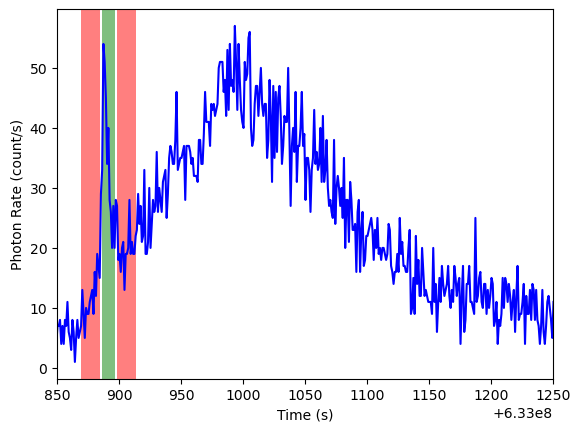
\includegraphics[scale=0.5]{109_ts_zoomout.png}
    \captionof{figure}{TimeSeries visualization of the detected peak in Figure \ref{img:peakA}, x-axis adjusted to show most of the flare ($t$ = 633000850 to 633001200).}
  \end{minipage}
\end{figure}

\begin{figure}[h]
    \centering
    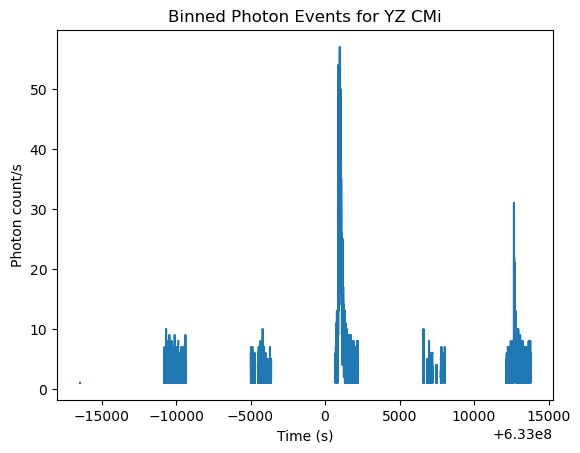
\includegraphics[scale=0.52]{109_ts.png}
    \caption{TimeSeries of entire binned photon data for Star B (YZ CMi) without SNR analysis.}
    \label{img:tsB}
\end{figure}

\begin{figure}[h]
    \centering
    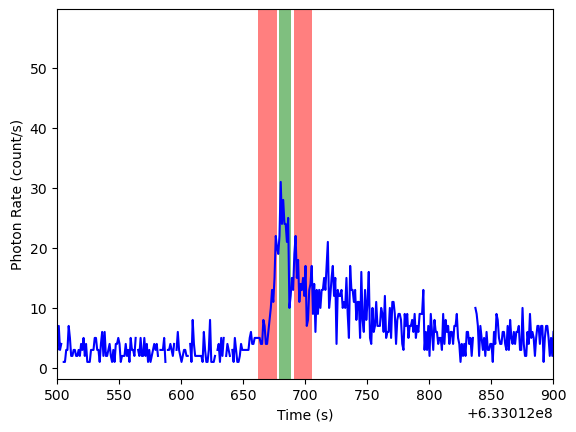
\includegraphics[scale=0.52]{109_ts_another.png}
    \caption{TimeSeries of the other, smaller, observed peak in photon event data for YZ CMi.}
    \label{img:tsAnother}
\end{figure}

\begin{multicols}{2}

Particularly large flares are potentially visible by eye, without using SNR analysis in the time domain (Figure \ref{img:tsB}). It is also easy to identify another between roughly $t$ = 633012000 and 633013000, pictured in Figure \ref{img:tsAnother}. However, identifying flares by eye is time- and power-consuming as each star must be individually analyzed, for potentially many terabytes of data. This reveals the appeal of Flare Finder, as the entire process is automated from beginning to end, with flare candidates and visualizations directly reported and saved locally. For both observed spikes in photons/second in Figure \ref{img:tsB}, those timestamps are returned without guesswork or estimation. 

\section{Summary and Possible Improvements}

To reduce bias in NUV data for observed flares in M-dwarfs, Flare Finder is an algorithm designed to blindly search for flares and output flare star candidates in \textit{Swift} UVOT event data. It iterates in polynomial time over any inputted UVOT event data and calculates SNRs in the time domain to determine timestamps of significantly higher photon output. When analyzing data from the \textit{Swift} UVOT with flares on YZ CMi, the algorithm accurately reported the timestamps of both and provided other visualizations, including histograms of the SNRs. 

Several small but persistent issues remain at hand, including noise distinction, the time window heuristic, and the SNR calculation over the time domain.
\begin{itemize}

\item \textbf{Noise distinction.} The current version of Flare Finder does not deal with high spikes of noise, as seen (potentially) in Figure \ref{img:zoomA}, and could mistake them as very short flares. 

\item  \textbf{Time window heuristic.} Flare Finder relies on an estimation for the length of the flare (e.g. 10 seconds), or several estimations (5 \textit{and} 10 seconds) to decrease processing time. This causes longer- or shorter-lasting flares to be ignored (e.g. in Figures \ref{img:zoomA} and 11). Optimizing the calculation process, or potentially using machine learning to choose better lengths for the time window, will increase Flare Finder's accuracy.

\item \textbf{SNR calculation.} By definition, the standard deviation of the distribution of SNRs for each star should be 1. However, when analyzing the data, it consistently measured a standard deviation of about 0.5, indicating something in the calculation process may be systematically affecting the SNR.

\end{itemize}

\section{Acknowledgements}
I would like to specially thank my mentor, Aaron Tohuvavohu, for dedicating the time and guidance to me for this project, helping to compile background resources, and providing valuable insight and knowledge on this research. I also extend thanks to the Institute for Computing in Research, and specifically Dr. Mark Galassi and Mr. José Medina-Hernandez for offering me this opportunity to complete this project.

\textit{Software}: Astropy (\cite{astropy:2013}; \citeyear{astropy:2018}; \citeyear{astropy:2022}), Jupyter Notebook (\cite{jupyter}), Numpy (\cite{numpy}), Pillow (\cite{pillow}), Scipy (\cite{scipy}).

\end{multicols}

\begin{center}
    \Large
    \textbf{References}
\end{center}

\printbibliography[heading=none]

\end{document}
